\documentclass{article}
\usepackage[utf8]{inputenc}
\usepackage[spanish]{babel}
\usepackage{listings}
\usepackage{graphicx}
\graphicspath{ {imagenes/} }
\usepackage{cite}

\begin{document}

\begin{titlepage}
    \begin{center}
        \vspace*{1cm}
            
        \Huge
        \textbf{Taller de Memoria del Computador}
            
        \vspace{0.5cm}
        \LARGE
        Proyecto de Invetigación
            
        \vspace{1.5cm}
            
        \textbf{Javier Andrés Mosquera Merchán}
            
        \vfill
            
        \vspace{0.8cm}
            
        \Large
        Despartamento de Ingeniería Electrónica y Telecomunicaciones\\
        Universidad de Antioquia\\
        Medellín\\
        Septiembre de 2020
            
    \end{center}
\end{titlepage}

\tableofcontents

\section{INTRODUCCIÓN}
Este documento es un desarrollo de respuestas investigativas, enfocadas en preguntas especificas del tema de memorias de un computador. Esto basado en un documento desarrollado por el profesor y jefe del departamento de ingenieria electronica de la universidad de Antioquia, Augusto Salazar, donde se describe el funcionamiento del computador y de que manera la memoria se involucra en cada proceso de dicho funcionamiento, además de describir el comportamiento de varios tipos de memorias que encontramos en un computador.\cite{referencia}

Las preguntas a responder son:

- Defina que es la memoria del computador.

- Mencione los tipos de memoria que conoce y haga una pequeña descripción de cada tipo.

-Describa la manera como se gestiona la memoria en un computador.

- ¿Qué hace que una memoria sea mas rapida que otra? ¿Por qué esto es importante?

\section{CONTENIDO} \label{contenido}
A continuación se presentara cada de las respuestas a cada pregunta presentadas en el documento guia.\cite{referencia}
Se aboradaran varias referencias de manera que haya una sintesis explícita y conjunta que responda cada pregunta.

\subsection{Definicion de Memoria del Computador}\label{pregunta1}
Para definir la memoria del computador no es necesario investigar mucho al respecto, una persona escogida al azar, y que a su vez haya vivido alguna experiencia cercana a un ordenador puede darnos una definición vaga que nos de mucha información sobre la memoria de un computador. Sin embargo, a un estudiante de las ciencias de la tecnologia no le basta con una respuesta de este tipo, para él es necesario, además de un concepto "desmenuzado", un soporte válido de la información que quiere obtener. Por ésta razón, es necesario adjuntar definiciones oficiales que me guien a dar una definición completa sobre la memoria de un computador.

(\ref{fig:almacenar})

\begin{figure}[h]
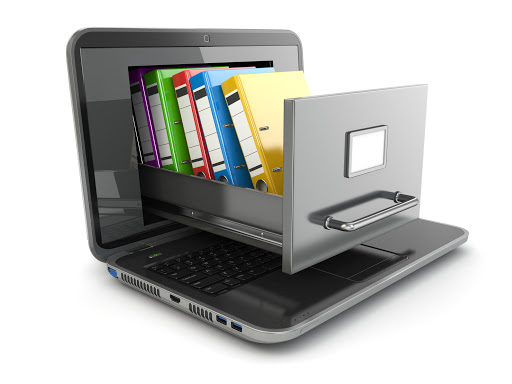
\includegraphics[width=4cm]{almacenar-informacion.jpg}
\centering
\caption{Almacenamiento de Informacion}
\label{fig:almacenar}
\end{figure}

Wikipedia, una pagina que brinda información a la comunidad, sobre cualquier tema, dice lo siguiente sobre la memoria:
"En informática, la memoria es el dispositivo que retiene, memoriza o almacena datos informáticos durante algún periodo de tiempo.1​La memoria proporciona una de las principales funciones de la computación moderna: el almacenamiento de información y conocimiento. Es uno de los componentes fundamentales de la computadora, que interconectada a la unidad central de procesamiento (CPU, por las siglas en inglés de Central Processing Unit) y los dispositivos de entrada/salida, implementan lo fundamental del modelo de computadora de la arquitectura de Von Neumann."\cite{wikipedia}

Ahora buscamos que dicen los fabricantes al respecto, Kingstone es uno de los fabricantes mas famosos de memorias en el mundo, y en su pagina web nos advirten sobre la diferencia entre memoria y almacenamiento, lo que nos dicen es: "Mientras la memoria se refiere a la ubicación de los datos a corto plazo, el almacenamiento es el componente de su computadora que le permite almacenar y acceder a datos a largo plazo. Usualmente, el almacenamiento se da en forma de una unidad de estado sólido o un disco duro. El almacenamiento le permite acceder y almacenar sus aplicaciones, sistema operativo y archivos por un tiempo indefinido.", entonces debemos tener cuidado con lo que llamamos memoria.\cite{kingstone}

Aunque es difícil encontrar mas definiciones generales con respecto a la memoria de un computador, sin que se refieran a algun tipo en especifico, adjuntare una definición de la memoria en general, esto con el objetivo de analizar si debemos tener restricciones en el lenguaje cuando llamamos un elemento como memoria.

Al teclear en google definiciones de la memoria, resulta que google tiene su propia seccion de definiciones elaborada por la universidad de Oxford donde nos dan las siguientes definiciones:
\begin{itemize}
    \item
    "Capacidad de recordar."\cite{google}
    \item
    "Imagen o conjunto de imágenes de hechos o situaciones pasados que quedan en la mente."\cite{google}
    \item
    "Dispositivo de una máquina donde se almacenan datos o instrucciones que posteriormente se pueden utilizar."\cite{google}
\end{itemize}

Finalmente con toda la informacion recopilada podemos, por fin, dar una buena definición de memoria del computador, es entonces, un sistema de  retención de datos o instrucciones, a corto o a largo plazo, los datos son representados por fenomenos fisicos, que serán utilizados e interpretados posteriormente por otros sistemas informáticos internos de la computadora; ésta información es la que permite superficialmente la interacción con el usuario. Guardar datos requiere de muchos procesos, ya que hay ambiguedades entre la maquina y el hombre, por lo que la memoria del computador debe dividirse en muchos subsistemas y es por ésto que existen diferentes tipos de memoria o tambien conocidos como dispositivos de almacenamiento.
Es importante recalcar que no hay problema en llamar a un dispositivo de almacenamiento como memoria, ya que la memoria guarda información, independientemente del tiempo, sin embargo, lo contrario no es posible, ya que el dispositivo de almacenamiento guarda informacion por un tiempo prolongado, y la perdida de esta informacion requiere permisos de usuario.

\subsection{Tipos de Memoria}\label{pregunta2}
Existen demasiados tipos de memoria, en la actualidad se ha avanzado mucho tanto en capacidad, como velocidad, además, como nos cuenta Augusto en su documento \cite{referencia}, las memorias tienen demasiadas funcionalidades, por lo que no todas cumplen con el mismo objetivo, sin embargo, las memorias se pueden clasificar en dos tipos: memorias volátiles y memorias NO volátiles.
\begin{itemize}
    \item
    MEMORIAS VOLÁTILES
    
    (\ref{fig:volatil})

    \begin{figure}[h]
    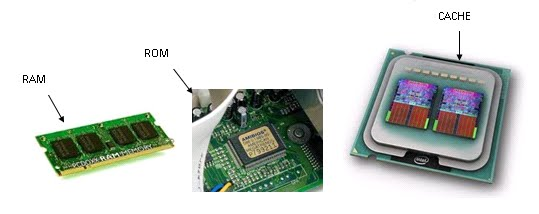
\includegraphics[width=4cm]{Volatiles.jpeg}
    \centering
    \caption{Ejemplos de Memorias Volatiles}
    \label{fig:volatil}
    \end{figure}
    
    Se denomina memoria volatil al dispositivo que pierde la informacion cuando se corta el fluido eléctrico. Como ejemplos de memorias volatiles tenemos:
    \begin{itemize}
        \item
        Memoria RAM(Random Access Memory): La memoria ram es un tipo de memoria que retiene su información por medio de capacitores, donde un capacitor cargado representa un 1 y un capacitor descargado representa un 0. Esta memoria tiene acceso aleartorio, es decir, que no es necesario recorrer la memoria hasta encontrar la información que se busca. Existen memorias ram dinamicas(DRAM) y estaticas(SRAM). La diferencia entre ambas es la forma de retener la informacion, la DRAM  utiliza una tecnología dinamica que le exige estar recargando la información, esta exigencia tiene un costo y es el de velocidad, mientras que la SRAM guarda la información con un arreglo de transistores, por esta razón no es necesario recargar la información, aún así, debe pagar un costo, y es de area superficial.
        
        \item
        Memoria Virtual: La memoria virtual es una solución que se le dio a los computadores sobre las limitaciones de memoria y posibilitar la ejecución de multiples programas previamente guardados, de este modo se evita que el computador te pida que cierres un programa para abrir otro. Se le llama volatil ya que lo que guarda son direcciones de memoria asociadas a procesos, una vez se pierde el flujo eléctrico el computador pierde los procesos y por ende las direcciones asociadas a esos procesos.
        
        \item
        Memoria Caché: La memoria cache es la mano derecha del procesador, es la memoria mas rápida y la de menos capacidad de almacenamiento, esta memoria tiene subdivisiones, permitiendo mayor velocidad a la subdivision que se encuentra al lado del procesador. Se encarga de guardar datos e instrucciones en calor, es decir, que estan en constante uso. El objetivo de esta memoria es dar la impresión de que las referencias a memoria se sirvan  a una velocidad muy cercana  a la del procesador.
    
    \end{itemize}
    
    \item
    MEMORIAS NO VOLÁTILES
    
    (\ref{fig:Novolatil})

    \begin{figure}[h]
    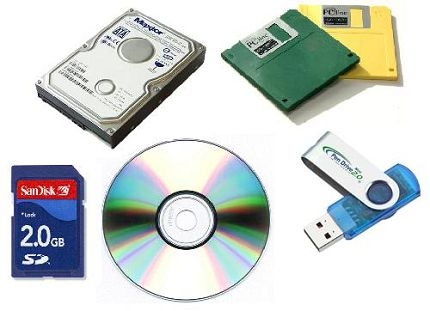
\includegraphics[width=4cm]{No-volatiles.jpg}
    \centering
    \caption{Ejemplos de Memorias NO Volatiles}
    \label{fig:Novolatil}
    \end{figure}
    
    Se denomina memoria volatil al dispositivo que pierde la información cuando se corta el fluido eléctrico. Como ejemplos de estas memorias tenemos los siguientes:
    \begin{itemize}
        \item
        Disco duro: Es la memoria encargada de guardar la mayor parte de información de un computador, puede llegar a tener capadidades de hasta 2 TB en referencias comerciales, lo que le cuesta en velocidad, es la memoria mas lenta del computador aún sabiendo que tecnologias actuales han llegado a velocidades extraordinarias. Es la encargada de guardar informacion como lo es el sistema operativo, programas y multimedia de forma permanente. Por esta razón es comunmente llamdo dispositivo de almacenamiento.
        
        \item
        Memoria ROM: Esta memoria es de solo lectura, y esta asociada mas al hardware que al software de un computador, ya que contiene los detalles de cada dispositivo interno del ordenador, como sus protocolos de comunicación y sus especificaciones.
        
        \item
        Memoria USB: La memoria usb es un dispositivo de almacenamiento permanente y extraible, es portatil y de area superficial relativamente pequeña. Es comunmente usada para guardar información multimedia y por esta razón tiene grandes capacidades de almacenamiento.
        
        
        \item
        CD o DVD: Son dispositivos de almacenamiento casi obsoletos, actualmente muchas marcas han retirado sus espacios de entrada en computadores, disminuyendo asi, el area superficial del ordenador. Cumplen las mismas funciones de una memoria USB, con limitaciones de capacidad.
    
    \end{itemize}
    
    
\end{itemize}

\subsection{Gestión de Memoria en un Computador}\label{pregunta3}
Basados en un articulo web de la universidad de Manizales \cite{UdeMa} y en el documento guia \cite{referencia}, podemos facilmente describir la gestión de memoria del computador.

Para empezar la gestión de memoria de un dispositivo informático consiste en mecanimos para asignar secciones de memoria a los programas que las solicitan, y a la vez, liberar las secciones de memoria que ya no se utilizan para que estén disponibles para otros programas. 

La parte del sistema operativo que administra la memoria se llama administrador de memoria y su labor consiste en llevar un registro de las partes de memoria que se estén utilizando y aquellas que no, con el fin de asignar espacio en memoria a los procesos cuando éstos la necesiten y liberándola cuando terminen.

La gestión de memoria tiene características y objetivos muy importantes en el funcionamiento correcto y preventivo. Entre ellas tenemos la protección la cual es el metódo encargado de controlar el uso de memoria en una computadora, de esta manera evita que un proceso acceda a un espacio de almacenamiento que no se le fue asignado. 
Por otro lado tenemos la memoria compartida, encargada de reutilizar espacios de memoria que ya fueron utilizados y en tiempo real son necesitados, esto permite agilizar los resultados y hacer mas en menos tiempo.
Tambien se cuenta con la organizacion, primero existe la llamada organización lógica quien permite que los programas se escriban como módulos compilables y ejecutables por separado. Pero por separado esta la organización fisica, la memoria suele dividirse en un almacenamiento primario de alta velocidad y uno secundario de menor velocidad.  La gestión de memoria del sistema operativo se ocupa de trasladar la información entre estos dos niveles de memoria.

Pero, ¿Qué pasa cuando pulsamos el botón de encendido?. 
Cuando el circuito integrado encargado de verificar la correcta alimentación del sistema, recibe la señal de encendido, inmediatamente envia la señal al procesador de que es inminente el encendido, por lo tanto procede a buscar las instrucciones en la memoria ROM; intrucciones que dan un recorrido entero por el equipo verificando el estado del hardware, cuando certifica que todo esta en excelente estado se carga el programa principal del computador, la BIOS, un programa que se encuentra incorporado en un chip de la placa base, y es quien se encarga de  realizar las funciones básicas de manejo y configuración del ordenador. Se Puede afirmar que es un conjunto de rutinas y procedimientos elementales que coordinan y manejan los elementos de hardware básico.
Por lo tanto este programa verifica cuantas particiones hay en el disco duro y que sistemas operativos se encuentran en cada una de ellas, si hay mas de un S.O. debe existir una interfaz que muestra en pantalla las opciones posibles de iniciar, si solo hay uno entonces inmediatamente inicia con éste. Una vez hecho este paso, se carga el sistema en la memoria RAM, o por lo menos sus funciones básicas, por esta razón, mientras se muestra el logo de espera de un programa o imagen, el cursor del mouse se puede mover tranquilamente y sin problemas por la pantalla; mientras todo esto pasa, la memoria caché hace funciones básicas mucho mas necesarias, como guardar direcciones de memoria donde se encuentran los elementos del sistema operativo que serán cargados en la memoria RAM o guarda archivos de texto con instrucciones de verificación del propio software, en paralelo el microprocesador hace calculos a velocidades inimaginables para poder atender todas las interrupciones del sistema; antes de terminar de cargar completamente el sistema operativo, hay un paso de verificación, donde el usuario que utilizará el computador se logea y estas credenciales se guardan en memoria RAM para tener a la mano posibles permisos en un futuro y agilizar los procesos, sin esperar que el usuario se logee nuevamente. Paso seguido, el sistema carga los archivos de autorun, estos archivos contienen las instrucciones de carga de programas y funciones necesarias para el usuario, como mostrar la barra de tareas, la imagen que el usuario escogió como fondo de pantalla, o los iconos de los programas disponibles para cargarsen. Una vez hecho ésto, las memorias y dispositivos ya saben como comunicarsen entre si cuando se necesiten mutuamente, y a partir de este momento todas quedan a la espera de las peticiones del usuario, que es quien dirige las instrucciones el resto del tiempo.

\subsection{¿Qué hace que una memoria sea más rápida que otra?
            ¿Por qué esto es importante?}\label{pregunta4}
Hay muchos factores que determinan la velocidad de una memoria, como por ejemplo, la forma en que estan fabricados, el modo de acceso a la información, y la comunicación que tiene con el microprocesador.
Ya se habia mencionado de que manera pueden estar fabricada la memoria RAM, por medio de capacitores o por transistores. Además que la DRAM está fabricada con capacitores y la SRAM con transistores, por esto la SRAM es mas rápida que la DRAM. Por otro lado la memoria caché siendo la mas rápida de las memorias esta constrida con memorias SRAM en su interior.
Ahora el disco duro es el mas lento de las memorias, ya que depende de los giros del disco, que a su vez, los giros dependen del radio, es decir que entre mayor se la capacidad, menor será la velocidad.
También se habia mencionado que al acceder a una memoria de manera aleartoria, agilizaría el proceso de adquisición de información, mientras que si es un acceso direccionado, se debe utilizar mas tiempo para obtener los datos. Entonces mientras mas grande sea el dispositivo, mas tiempo tomará para cualquier petición.
Por último y no menos importante, la comunicación, el bus de datos es muy importante a la hora de obtener la información, ya que pueden haber "tacos" o aglomeración de peticiones. Además el ancho del bus de datos permite, duplicar y hasta cuadriplicar el envío de información lo que intuitivamente nos haría pensar que se reduce en la misma proporción el tiempo de ejecución. No es lo mismo un bus de datos de 8 bits que uno de 64 bits.

Analizar estos temas es esencial en el diseño del computador, ya que la demanda se puede ver perjudicada por esta razón. Vivimos en una epoca donde la información se volvió vital en nuestras vidas, por lo tanto, mientras mas rápido accedamos a ella, mejor productividad tendremos en la vida académica o laboral. 
Desde una perspectiva un poco mas amplia, podríamos pensar en un avión que viaja de un continente a otro; sabemos que cada avión tiene su sistema de comunicación, y que estos sitemas son controlados por computadoras, entonces si una computadora no es lo suficientemente rapida como para procesar la información que se le envía, el piloto no tendría la información de la tormenta que esta próximo a atravesar, o no estaría enterado de que otro avión converge a la misma dirección que viaja él. Estos errores de sistemas pueden provocar catastrofes de magnitudes extraordinarias.
Es importante saber el papel que juega una memoria en la vida contemporanea, y mas aún, el rol que jugara en los tiempos venideros, donde la tecnología inundará cada rincón del planeta.



\vspace{10.5cm}



\section{Conclusión} \label{conclulsion}
\begin{itemize}
    \item 
    Es muy importante conocer lo que hay detrás de cada click en nuestras vidas, en muchos casos, cuando el computador esta lento, el usuario comienza abrir todo y dar click a cuanto icono se le aparezca para "agilizar" el computador, ésto porque ignora el "detras de escenas" e intuitivamente se imagina que asi logrará hacerlo entrar en razón, cuando realmente lo que hace es copándolo de mas tareas e interrupciones del sistema, generando mas pérdida de tiempo y mayor estrés para entregar el trabajo a su jefe. A su vez, el estrés le aumenta la presión arterial, aumentando las posibilidades de un paro cardiaco inmediato. Es increíble lo que hay detrás de la cadena de sucesos que genera un click.
    \item
    Al visualizar nuestra vida como programadores de sistemas informáticos, es indispensable conocer los recursos que poseemos y como podemos hacer uso de ellos. Como ingenieros, nuestra tarea es solucionar problemas de la manera mas eficiente, pero, ¿Cómo pretendemos hacer un programa que diagnostique un paciente con COVID-19, si al analizar el tercer paciente no queda espacio suficiente en la memoria?.
    \item
    Tan sencillo como el fastidioso mensaje de "No queda espacio disponible en el dispositivo" a la hora de descargar un programa que te salvará el parcial virtual, entonces, no tienes porque gastar tiempo, yendo hasta configuracion-almacenamiento-borrar memoria caché. Conocer los diferentes tipos de memoria nos puede ayudar a resolver problemas simples de la vida cotidiana, en nuestro constante uso de sistemas informáticos.
    
\end{itemize}


\bibliographystyle{IEEEtran}
\bibliography{references}

\end{document}

